\section{CSS_Layout}\label{sec:CSS_Layout}

\begin{frame}
    \frametitle{El modelo de caja}

    Hasta ahora solo cambiamos cómo se ven los elementos en el sitio. Sin 
    embargo, una de las cosas más potentes de CSS es que también podemos 
    cambiar cómo se organizan. Vamos a cambiar el \emph{layout} del sitio.

    En CSS, todos los elementos están en cajas. Estas cajas tienen 4 partes:

    \begin{itemize}
        \item El contenido: Lo que metemos en los elementos. Texto, imágenes, 
              otros elementos, etc.
        \item \emph{Padding}: Justamente es un relleno alrededor del contenido. 
              Suele verse como parte del elemento.
        \item Borde: El espacio entre el padding y el margen. Marca el límite 
              del elemento.
        \item Margen: El espacio entre el elemento y otros elementos. En general 
              no se ve como parte del elemento. Cuando hay dos elementos juntos sus 
              márgenes se suman.
    \end{itemize}

    En ese orden desde adentro hacia afuera. 

\end{frame}

\begin{frame}
\frametitle{El modelo de caja}

    Por defecto, el ancho y alto de un elemento se calculan solo en base al 
    contenido, por lo que hay que sumar el padding, borde y margen para 
    conseguir el tamaño total de la caja. La regla 
    \inlinecode{box-sizing: border-box} permite cambiar esto para que se calcule 
    en base al contenido, padding y borde, sin incluir el margen.

    \begin{figure}[h]
        \centering
        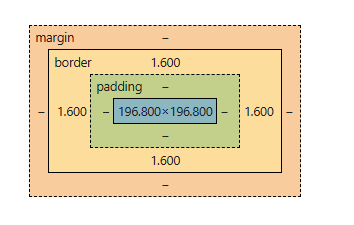
\includegraphics[width=0.6\textheight]{../images/box_model.png}
        \caption{El modelo de caja}
    \end{figure}

\end{frame}

\begin{frame}
\frametitle{Manipulando la caja}

    Ahora que entendemos cómo están compuestos los elementos, empezemos 
    a cambiarles la forma. El padding y el márgen tienen 
    propiedades que permiten cambiarlos en cualquier dirección:

    \begin{itemize}
        \item \inlinecode{padding: valorParaLas4Direcciones}
        \item \inlinecode{padding: valorVertical valorHorizontal}
        \item \inlinecode{padding: arriba derecha abajo izquierda}
    \end{itemize}
    
    Las mismas versiones existen para \inlinecode{margin}. También existen propiedades 
    específicas para cada lado (por ej. \inlinecode{padding-top}), no hace 
    falta setear las cuatro direcciones siempre.

    La propiedad del borde es un poco distinta, pero también tiene propiedades 
    específicas que permiten tocar cada lado por separado.

    \begin{itemize}
        \item \inlinecode{border: grosor estilo color}
    \end{itemize}

\end{frame}

\begin{frame}
\frametitle{Manipulando la caja}

    También podemos cambiar el tamaño del contenido! O por lo menos intentarlo.
    Las propiedades \inlinecode{width} y \inlinecode{height} hacen exactamente eso. 
    Como dijimos antes, si \inlinecode{box-sizing} es \inlinecode{border-box},
    los valores de estas propiedades incluyen al padding y el borde.

    Acá entramos un poco en terreno tormentoso. Si el tamaño que le damos 
    al contenido no es suficiente, el contenido podría escaparse del contenedor, 
    cosa que se conoce como \emph{overflow}. Si el tamaño que le damos es demasiado, 
    nos van a quedar agujeros medio raros.

    También existen propiedades \inlinecode{min-width} y \inlinecode{max-width} 
    (y lo mismo para height) que limitan los valores de las propiedades anteriormente 
    mencionadas. Ahora, ¿por qué existen esas propiedades? ¿Por qué alguien pondría 
    un valor de width mayor al de max-width?

\end{frame}

\begin{frame}
\frametitle{Unidades y un flash de diseño receptivo (\emph{responsive})}

    Más atrás mencionamos muy al pasar algunas unidades que se usan para los 
    valores de las propiedades. Estas unidades se distinguen en dos categorías:

    \begin{itemize}
        \item Absolutas: Indican la misma magnitud sin importar en qué contexto 
              aparezcan*. Son cm, mm, Q ($\frac{1}{4}$mm), in, pc, pt y px.
        \item Relativas: La magnitud que representan depende del contexto. Más 
              detalles en la siguiente diapo.
    \end{itemize}

    Volviendo a \inlinecode{width} y \inlinecode{max-width}, alguien podría 
    definir el ancho de un elemento con una unidad relativa pero después ponerle 
    un límite con una unidad absoulta.

\end{frame}

\begin{frame}
\frametitle{Unidades relativas}

    Las unidades relativas son las siguientes:

    \begin{itemize}
        \item em se refiere al tamaño de la fuente del elemento al que se le 
              aplica la regla*. \inlinecode{2em} es el doble de ese tamaño.
        \item rem se refiere al tamaño de la fuente del elemento raíz.
        \item vh se refiere a la altura del \emph{viewport}, el rectángulo en el 
              que se está mostrando el sitio. \inlinecode{1vh} es 1\% de ese tamaño. La 
              versión para el ancho es vw. Ver las versiones con s, l y d.
        \item vmin la más chica entre vh y vw. vmax es la más grande.
        \item Los porcentajes se refieren a un porcentaje de la propiedad en el 
              elemento padre. Por ejemplo: \inlinecode{width: 50\%} representa 
              la mitad del ancho que el elemento padre.
        \item fr se usa para específicamente para grids.
    \end{itemize}

    Hay unas cuántas más mucho más específicas pero no son muy comunes.

\end{frame}

\begin{frame}
\frametitle{Posición}

    Así como podemos cambiar la forma de los elementos, también podemos cambiar 
    dónde se ubican. La propiedad \inlinecode{position} define la forma en la 
    que los elementos se ubican en el sitio. Las propiedades \inlinecode{top}, 
    \inlinecode{bottom}, \inlinecode{left} y \inlinecode{right} mueven al elemento 
    de distintas formas según el valor de \inlinecode{position}. Dichos valores son: 

    \begin{itemize}
        \item \inlinecode{static}: El valor por defecto.
        \item \inlinecode{relative}: El elemento se posiciona relativamente a la 
              posición que le tocaría normalmente. Sigue afectando a otros elementos.
        \item \inlinecode{absolute}: El elemento se posiciona relativamente al ancestro 
              posicionado más cercano. Si ningún ancestro fue posicionado entonces es 
              relativo al viewport. Deja de afectar a otros elementos.
        \item \inlinecode{fixed}: Como absolute pero directamente es relativo al viewport.
        \item \inlinecode{sticky}: Funciona raro. Similar a relative, pero cuando quedaría 
              afuera por scrollear, se pega al tope.
    \end{itemize}

\end{frame}

\begin{frame}
\frametitle{Flexbox y grids. La propiedad \inlinecode{display}.}

    La propiedad \inlinecode{position} se usa para acomodar elementos de forma 
    muy específica. Muchas veces, lo que queremos es acomodar varios elementos 
    entre sí y de acuerdo a la caja que los contiene. Ahí surgen las \emph{grids} y 
    las \emph{flexible boxes}.

    Una grid se usa para partir un contenedor en secciones rectangulares. Se puede 
    partir en tantas secciones como uno quiera y pueden tener cualquier tamaño. Es 
    como una especie de mondrian.

    Una flexible box se usa para acomodar elementos de forma que cambien sus tamaños 
    acorde a la cantidad de espacio que haga falta. Son tan útiles que suelen estar 
    por todos lados.

    Un elemento se pone en modo grid o flexbox usando la propiedad \inlinecode{display} 
    con los valores \inlinecode{grid} y \inlinecode{flex} respectivamente. Hasta ahora 
    no la habíamos mencionado, pero esa propiedad también puede definir si el elemento 
    es \inlinecode{inline} o \inlinecode{block}. También se le puede dar el valor 
    \inlinecode{none} para sacar el elemento del sitio.

\end{frame}

\begin{frame}
\frametitle{Grid}

    % Cosas sobre grid

\end{frame}

\begin{frame}
    \frametitle{Flexbox}

    Como el nombre lo indica, un contenedor flexbox trata a sus elementos hijos 
    como cajas de espaciado (y a veces tamaño) adaptable al espacio disponible. El eje principal 
    sobre el cual se posicionan se define con la propiedad \inlinecode{flex-direction}, que puede
    ser \inlinecode{row}, \inlinecode{column}, o cualquiera con \inlinecode{-reverse} al final. 

    Para el posicionamiento, desde el contenedor usamos \inlinecode{justify-content} para controlar 
    posicion de elementos en el eje principal. Esto incluye el espacio entre elementos. 
    Algunas posibilidades son:  
    
    \begin{itemize}
        \item \inlinecode{start}, \inlinecode{end}, \inlinecode{center}: Elementos en la posición 
            indicada y "pegados", separados solo por sus margenes
        \item \inlinecode{space-between}: Aleja los elementos lo más posible, usando todo el espacio
        \item \inlinecode{space-evenly}: Similar al anterior, dejando espacio también con los bordes
    \end{itemize}
    
    \inlinecode{align-items} hace lo mismo en el eje opuesto, sin poder definir espaciado que no 
    tendría sentido.

\end{frame}

\begin{frame}
    \frametitle{Flexbox}
    
    Como alternativa a tener que esconder cosas en caso de overflow, podemos usar \inlinecode{flex-wrap}, 
    definiendo que los elementos se posicionen en una segunda fila o columna si no entran, 
    que permite automáticamente adaptarse a pantallas de distintos tamaños.

    En este caso, align-content nos dice como alinear la segunda fila o columna. Funciona igual que
    el \inlinecode{justify-content} en el otro eje. 

    También es posible indicarles a los elementos que se estiren a ocupar cierta proporción del 
    espacio que sobra usando \inlinecode{flex}.

    Hay otras propiedades de flex que modifican otros detalles del posicionamiento, que siempre
    pueden buscar si les interesa.

\end{frame}

\begin{frame}
    \frametitle{Ejercicio - }
    
    % Ejercicio de posicionamiento

\end{frame}

\begin{frame}
    \frametitle{Ejercicio - }

    % Ejercicio de flex y grid

    \href{https://css-tricks.com/snippets/css/a-guide-to-flexbox/}{Cheatsheet de flexbox}

    \href{https://grid.malven.co/}{Cheatsheet de grid}

\end{frame}